\section{Resultados y discusión}

Se presentan los resultados obtenidos a partir de las medidas de voltaje y desfasaje realizadas en el circuito RC en escalera, así como la respuesta del cable coaxial bajo tres condiciones de impedancia diferentes. En primer lugar, se construyeron diagramas de Bode con los datos obtenidos de la configuracion en escalera de RC, tanto para las medidas variando el nodo del circuito a una frecuencia constante, como para las medidas variando la frecuencia con nodo fijo. A partir de estos diagramas se obtuvo la constante característica del circuito \(\tau\). Asimismo se realizo un diagrama de Nyquist a partir de medidas realizadas sobre el primer nodo, variando la frecuencia, con el objetivo de comprobar el comportamiento del arreglo. 


\subsection{Circuito RC en escalera}

De acuerdo con la ecuación \eqref{eq:voltajePulso}, la amplitud de la señal decae exponencialmente con el nodo como $e^{kz}$ y presenta un corrimiento de fase proporcional a $kz$, con $k = \sqrt{\frac{\omega RC}{2}}$. Esto implica que el logaritmo del módulo y la fase deben depender linealmente tanto de $z$ como de $\sqrt{\omega}$, lo cual permite obtener $\tau=RC$ a partir de ajustes lineales. 

\subsubsection{Medidas a frecuencia constante}

 En la \autoref{fig:bode_z} se presenta el diagrama de Bode obtenido al variar el nodo a una frecuencia fija, así como los ajustes lineales realizados sobre los datos. Se observa que $20\log_{10}(H)$ decrece linealmente
     con el nodo $z$, mientras que la fase $\varphi$ aumenta de forma lineal, lo que es coherente con lo esperado para un circuito RC en escalera. Sin embargo, se puede observar una tendencia, en los nodos superiores, a alejarse del comportamiento predicho debido a una falla en la aproximación del circuito RC como escalera infinita, resultando en un aumento de la pendiente del ajuste.
     Mediante ajustes lineales se obtuvo una pendiente $m_H= -0.307(4)$ para el módulo y una pendiente $m_\varphi = 0.302(6)$ para la fase. Utilizando estas pendientes se calculó una constante de tiempo $\tau_H = 6.0(2)\times 10^{-4}$ \si{\second} y
      $\tau_{\varphi}=6.2(2)\times 10^{-4}$\si{\second} consistentes con el valor teórico calculado a partir de los componentes del circuito,
       $\tau_{\text{ref}} = \text{RC} = 5.9(4) \times 10^{-4}$ \si{\second}.  

\begin{figure}[H]
    \centering
    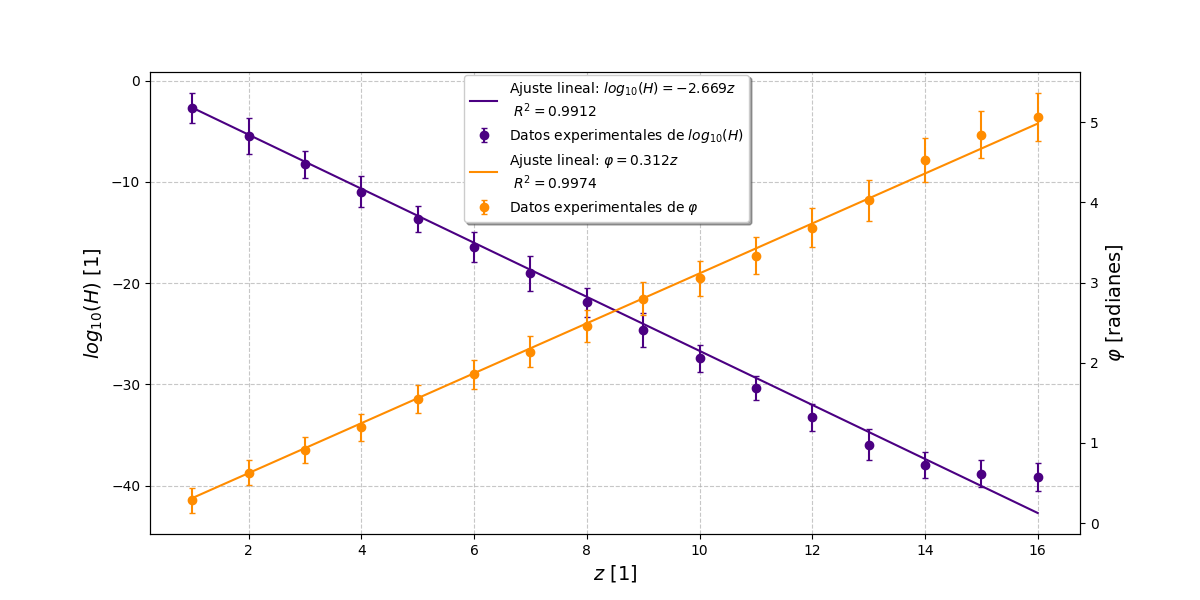
\includegraphics[width=0.5\linewidth]{gráficos/bode piola constante.png}
    \caption{Diagrama de Bode a frecuencia constante. En violeta se muestran los datos correspondientes al logaritmo del módulo, en naranja se presentan los datos correspondientes a la fase en radianes. Para ambos se observa un comportamiento lineal con respecto al nodo $z$. La línea violeta corresponde al ajuste lineal realizado sobre el logaritmo del módulo, mientras que la línea naranja corresponde al ajuste lineal realizado sobre la fase. Estos ajustes permitieron obtener valores de $\tau$, siendo $\tau_H = 6.0(2)\times 10^{-4}$ \si{\second} el obtenido a partir del módulo y $\tau_{\varphi}=6.2(2)\times 10^{-4}$\si{\second} el obtenido a partir de la fase.}
    \label{fig:bode_z}
\end{figure}


\subsubsection{Medidas en un punto fijo del circuito}

Se presenta en la \autoref{fig:bode_w} el diagrama de Bode construido a partir de tomar la tensión en un nodo fijo $z=6$ y variar la frecuencia, tanto como el ajuste realizado sobre los datos obtenidos. Nuevamente se observa un comportamiento lineal en los datos del módulo y la fase. A partir de las pendientes de los ajustes se obtuvieron los valores $\tau_H=6.7(9)\times 10^{-4}$\si{\second} y $\tau_{\varphi}=5.4(7)\times 10^{-4}$\si{\second}. Estos valores son consistentes con el valor teórico, lo que refuerza la validez del modelo utilizado para describir el comportamiento del circuito RC en escalera. En este caso, las incertidumbres asociadas a las medidas son mayores que en el caso de las medidas a frecuencia constante, lo cual puede deberse a errores experimentales relacionados con la medición de la fase para las distitas frecuencias.

\begin{figure}[H]
    \centering
    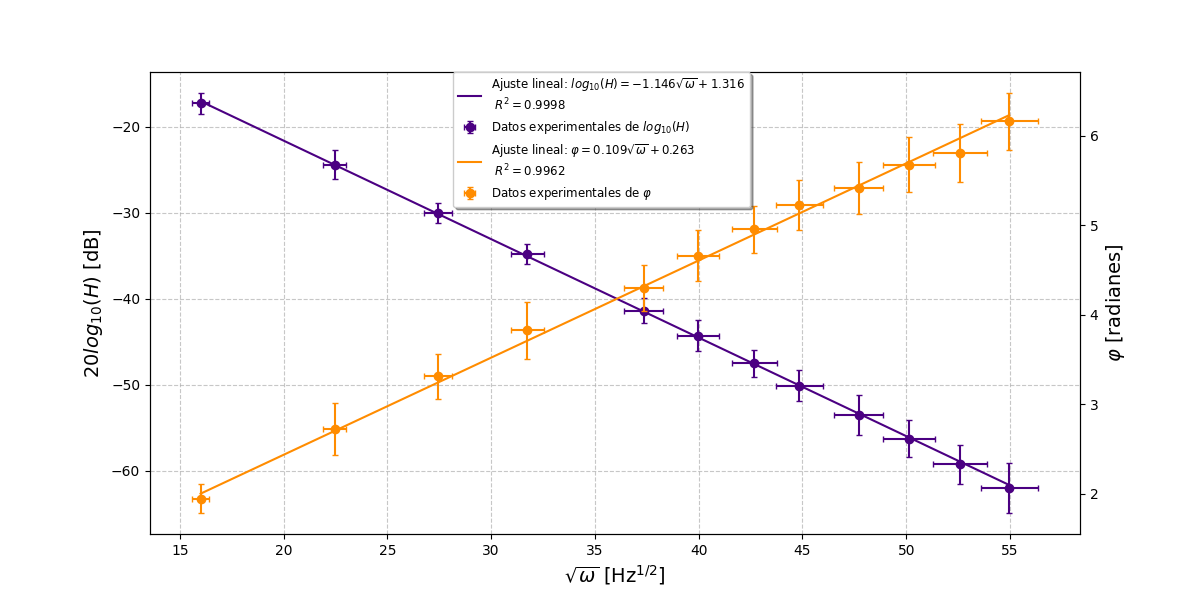
\includegraphics[width=0.5\linewidth]{gráficos/bode piola variable.png}
    \caption{Diagrama de Bode para las medidas dejando el nodo fijo. En violeta se muestran los datos correspondientes al logaritmo del módulo, en naranja se presentan los datos correspondientes a la fase en radianes. Para ambos se observa un comportamiento lineal con respecto a $\sqrt{\omega}$. La línea violeta corresponde al ajuste lineal realizado sobre el logaritmo del módulo, mientras que la línea naranja corresponde al ajuste lineal realizado sobre la fase. Estos ajustes permitieron obtener valores de $\tau$, siendo $\tau_H=6.7(9)\times 10^{-4}$\si{\second} el obtenido a partir del módulo y $\tau_{\varphi}=5.4(7)\times 10^{-4}$\si{\second} el obtenido a partir de la fase.}
    \label{fig:bode_w}
\end{figure}


Finalmente, se realizó un promedio ponderado con los valores obtenidos de $\tau$ a partir de las medidas a frecuencia constante y a nodo fijo, obteniendo un valor de $\tau_{\text{promedio}} = 6.1(1)\times 10^{-4}$ \si{\second} consistente con el valor de referencia.

\subsubsection{Impedancia Z del sistema}

Con el objetivo de comprobar el comportamiento del circuito RC en escalera, se construyó un diagrama de Nyquist a partir de las medidas 
    realizadas, de la misma manera que para el nodo 6, en el primer nodo. Asimismo, se calculó de manera analítica la curva teórica de la impedancia para el caso de un circuito RC en escalera de 16 nodos. En la \autoref{fig:Nyquist} se presentan ambos diagramas. Es posible observar que a frecuencias bajas la curva teórica predice el comportamiento real del circuito, mientras que a frecuencias altas pierde precisión. 

    \begin{figure}[H]
    \centering
    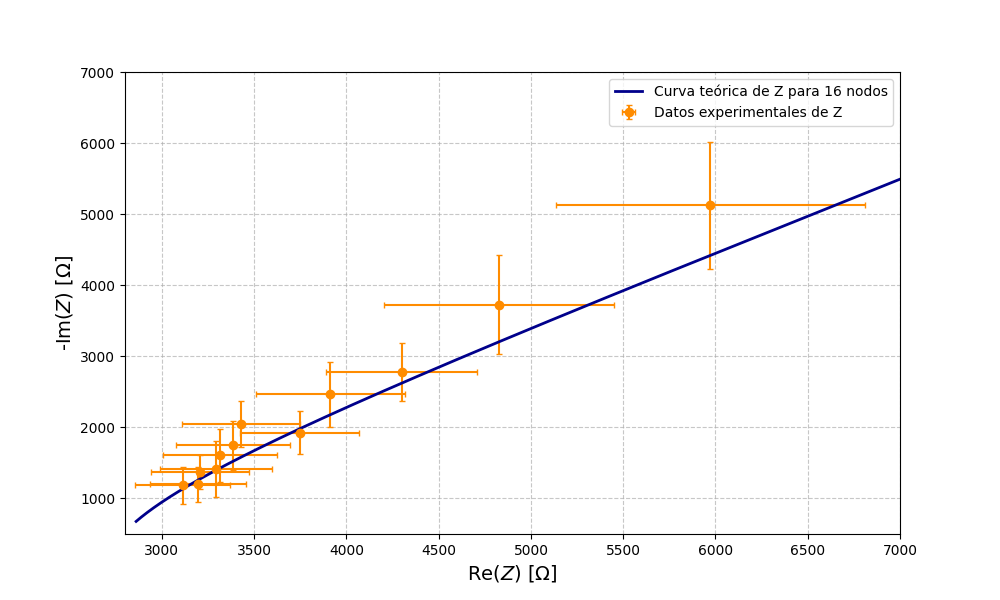
\includegraphics[width=0.5\linewidth]{gráficos/Nyquist_Z.png}
    \caption{Diagrama de Nyquist obtenido a partir de las medidas experimentales para el circuito RC en escalera junto con la curva teórica. En naranja se muestran los datos experimentales, mientras que en azul se presenta la curva teórica. Se observa que a frecuencias bajas la curva teórica pasa por todos los puntos experimentales, mientras que a frecuencias altas tiende a alejarse de los mismos.}
    \label{fig:Nyquist}
\end{figure}


\subsection{Cable coaxial}

En esta parte del experimento se analizó la propagación de pulsos en un cable coaxial bajo distintas condiciones de impedancia: Impedancia nula (cortocircuito), impedancia infinita (circuito abierto) e impedancia igual a la característica del cable. Las mediciones se realizaron con un osciloscopio, donde la señal superior corresponde a la señal de entrada (onda incidente) y la inferior a la señal de salida (onda reflejada).
Como se observa en la \autoref{fig:Coaxial_infinito}, para el caso de resistencia infinita, la señal reflejada presenta la misma polaridad que la señal incidente. Es decir, el pulso reflejado coincide en forma con el pulso de entrada. Esto indica que el extremo del cable se comporta como un circuito abierto, donde no circula corriente. Bajo esta condición, la energía de la onda no puede disiparse, por lo que refleja completamente hacia la fuente idealmente con la misma amplitud, cosa que no es así pues el cable no es un elemento ideal y genera una disipación de energía. Este comportamiento es consistente con un coeficiente de reflexión igual a 1.

\begin{figure}[H]
    \centering

    % Parámetros editables
    \def\anchosubfigura{0.40\textwidth}
    \def\separacionvertical{0.2cm}

    % Fila superior
    \begin{subfigure}[b]{\anchosubfigura}
        \centering
        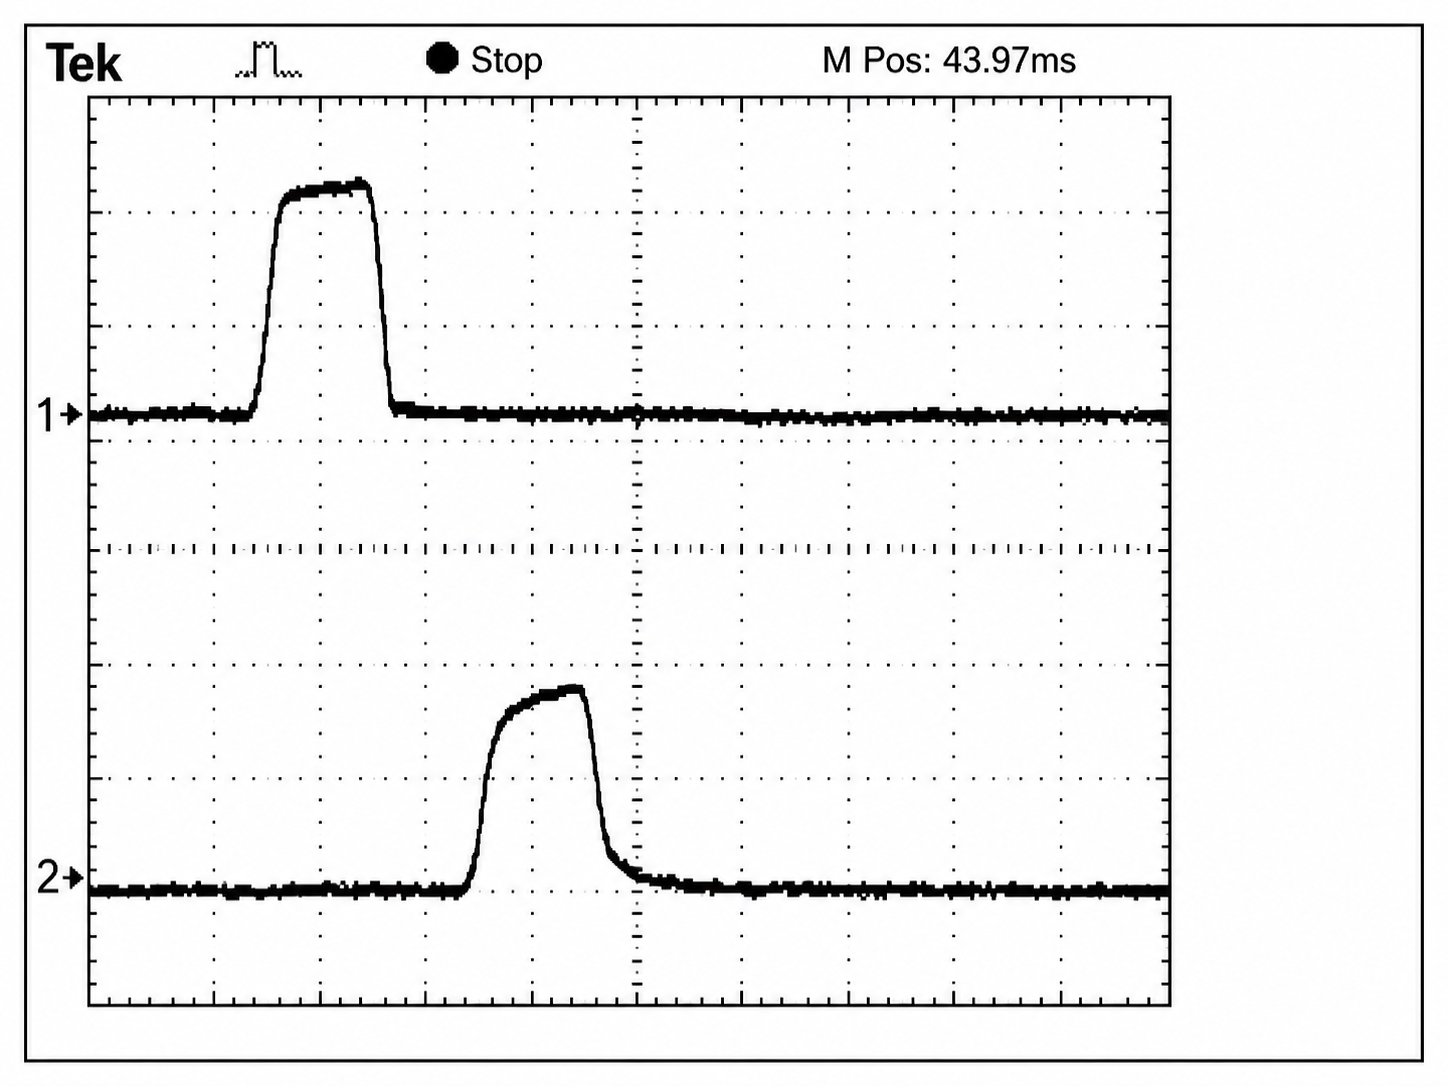
\includegraphics[width=\linewidth]{Figuras2/R_infinita.png}
        \caption{}
        \label{fig:Coaxial_infinito}
    \end{subfigure}

    \vspace{\separacionvertical}

    % Fila inferior
    \begin{subfigure}[b]{\anchosubfigura}
        \centering
        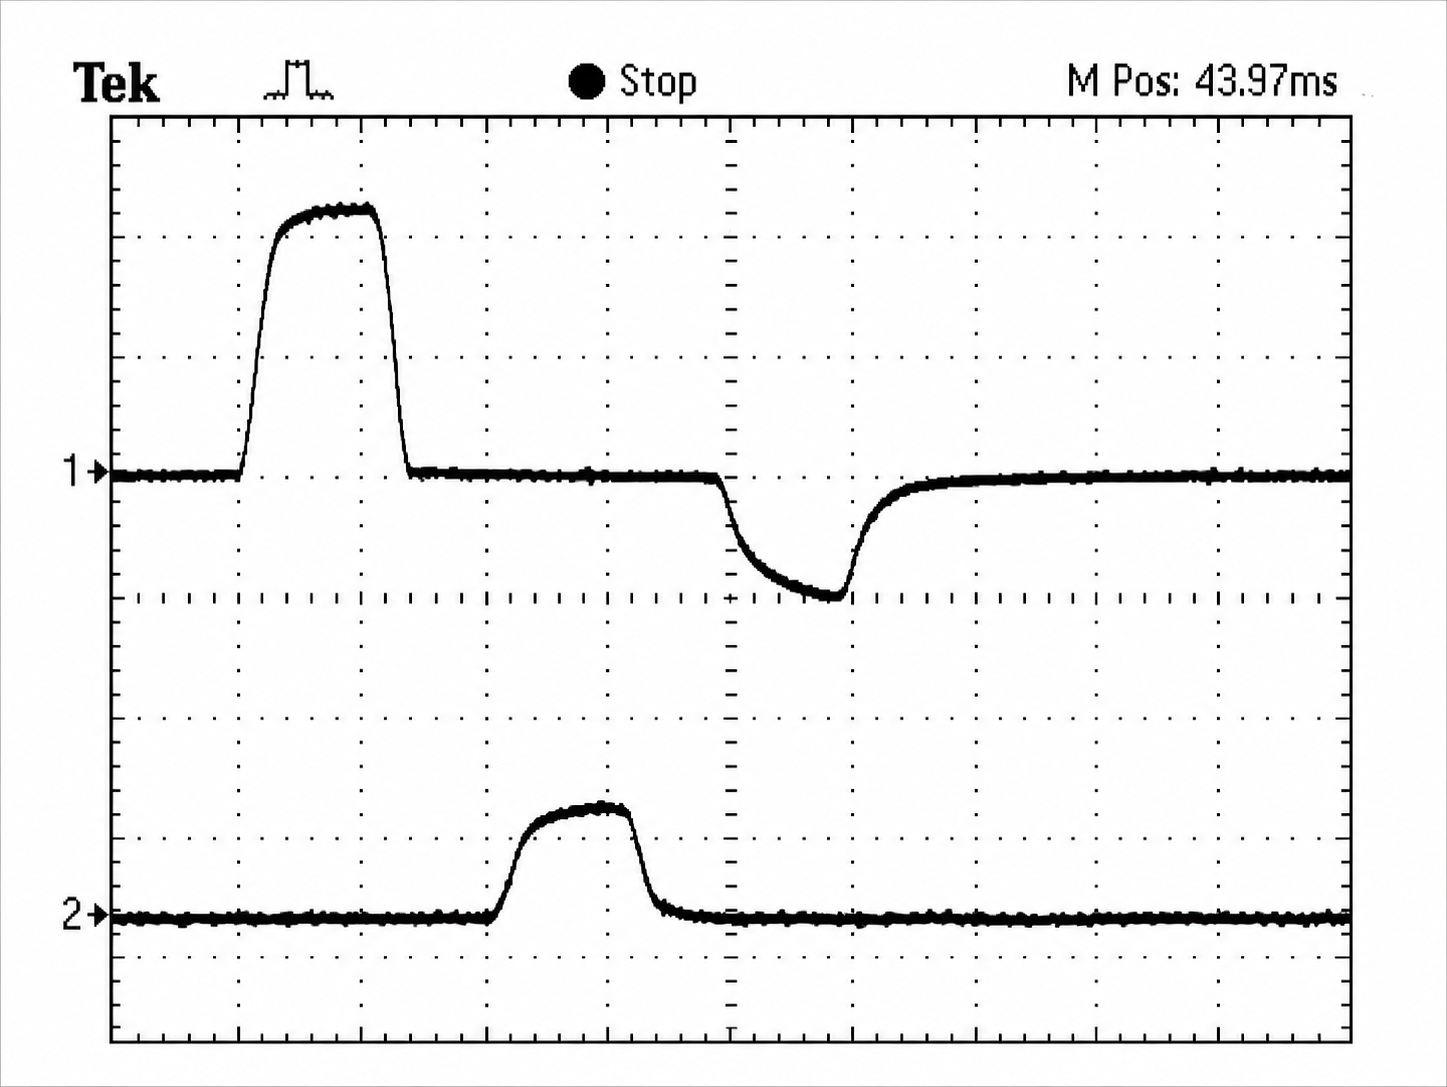
\includegraphics[width=\linewidth]{Figuras2/R_0.png}
        \caption{}
        \label{fig:Coaxial_nulo}
    \end{subfigure}
    \hfill
    \begin{subfigure}[b]{\anchosubfigura}
        \centering
        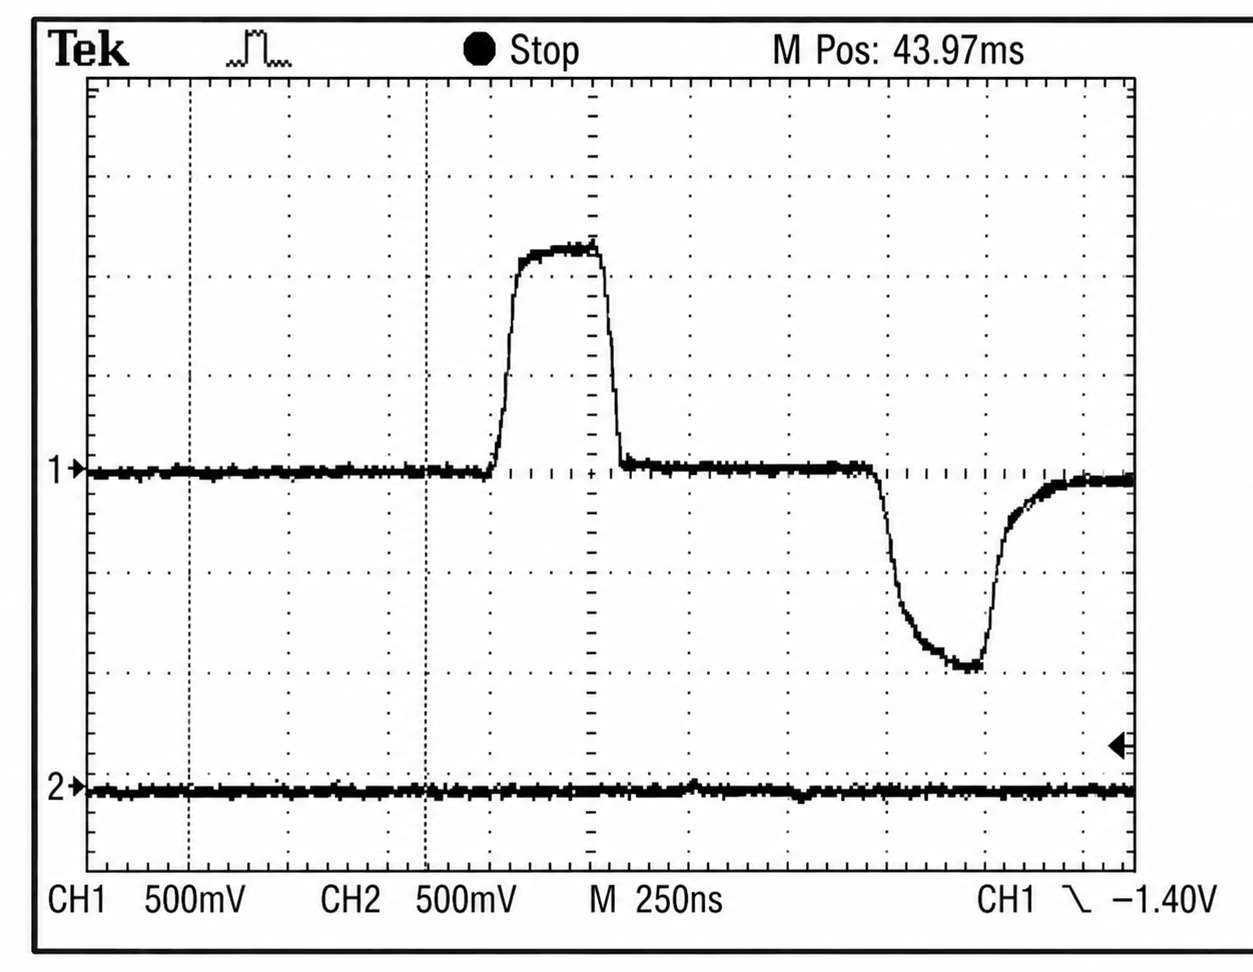
\includegraphics[width=\linewidth]{gráficos/R_Z0.png}
        \caption{}
        \label{fig:Coaxial_50}
    \end{subfigure}

    \caption{Respuesta del cable coaxial bajo distintas condiciones de impedancia. En los tres casos, el canal 1 mide el pulso incidente, así como un segundo pulso que carece de información importante para esta experiencia, y el canal 2 mide la suma del pulso incidente y el reflejado. En la figura (a) se muestra la respuesta para una impedancia infinita, en la figura (b) la respuesta para una impedancia nula, y en la figura (c) la respuesta para una impedancia igual a la característica del cable.}
    \label{fig:Coaxial_comparacion}
\end{figure}

%Respuesta del cable coaxial bajo distintas condiciones de impedancia. En la figura (a) se muestra la respuesta para una impedancia infinita,en la figura (b) se muestra la respuesta para una impedancia nula, y en la figura (c) se muestra la respuesta para una impedancia igual a la característica del cable.

En el caso de resistencia nula, se advierte la presencia de una señal que presenta una polaridad opuesta a la señal incidente en el canal de entrada. Este pulso invertido indica la existencia de una reflexión en el extremos del cable, característica de una terminación en cortocircuito, como se observa en la \autoref{fig:Coaxial_nulo}. La diferencia temporal entre ambas señales corresponde al tiempo de propagación de ida y vuelta en la línea. 
Bajo esta condición, la onda se refleja completamente hacia la fuente, pero con una inversión de fase de 180 grados, lo que resulta en una señal reflejada con polaridad opuesta a la señal incidente. Al igual que en el caso anterior, la amplitud de la señal reflejada no coincide exactamente con la señal incidente debido a las pérdidas energeticas en el cable. Este comportamiento concuerda con un coeficiente de reflexión igual a -1.


Finalmente, cuando la impedancia de la terminación es igual a la característica del cable (\(Z_C = 50(3)\) $\Omega$), no se observa señal reflejada. En esta condición, toda la energía de la onda incidente es absorbida, minimizando las reflexiones, como se puede ver en la \autoref{fig:Coaxial_50}. Idealmente, para este caso, el coeficiente de reflexión es nulo. 



En última instancia, se calculó la velocidad de propagación de la señal en el cable coaxial a partir del desfasaje temporal entre el pulso de entrada y el reflejado. Para el caso de impedancia infinita, se obtuvo una velocidad de propagación de \(v_{\infty} = 2.13(12) \times 10^8\) \si{\meter\per\second}, mientras que para el caso de impedancia nula se obtuvo \(v_0 = 2.08(11) \times 10^8\) \si{\meter\per\second}. Estos valores son consistentes entre sí y con la velocidad de propagación brindada por el fabricante, siendo esta de \(v_{\text{ref}} = 1.98(09) \times 10^8\) \si{\meter\per\second}, es decir el $66\%$ de la velocidad de la luz en el vacío.